\documentclass[11pt,aspectratio=169]{beamer}
\usepackage[utf8]{inputenc}
\usepackage[T1]{fontenc}
\usepackage{lmodern}
\usepackage[ngerman]{babel}
\usepackage{tikz}
\usetheme{Hannover}

\begin{document}
	\author{Joshua Bär und Michael Steiner}
	\title{Reed-Solomon-Code}
	\subtitle{}
	\logo{}
	\institute{OST Ostschweizer Fachhochschule}
	\date{26.04.2021}
	\subject{Mathematisches Seminar}
	\setbeamercovered{transparent}
	%\setbeamercovered{invisible}
	\setbeamertemplate{navigation symbols}{}
	\begin{frame}[plain]
		\maketitle
	\end{frame}
%-------------------------------------------------------------------------------	
\section{Einführung}
	\begin{frame}
		\frametitle{Reed-Solomon-Code:}
		\begin{itemize}
		\visible<1->{\item Für Übertragung von Daten}
		\visible<2->{\item Ermöglicht Korrektur von Übertragungsfehler}
		\visible<3->{\item Wird verwendet in: CD, QR-Codes, Voyager-Sonde, etc.}
		\end{itemize}
	\end{frame}
%-------------------------------------------------------------------------------	
\section{Polynom Ansatz}
	\begin{frame}
		\begin{itemize}
			\item Beispiel $2, 1, 5$ versenden und auf 2 Fehler absichern
		\end{itemize}
	\end{frame}
	\begin{frame}
		\frametitle{Beispiel}
		Übertragen von 
		${f}_2=\textcolor{blue}{2}$, ${f}_1=\textcolor{blue}{1}$, ${f}_0=\textcolor{blue}{5}$ 
		als $ p(w) = \textcolor{blue}{2}w^2 + \textcolor{blue}{1}w + \textcolor{blue}{5} $.
		
		\only<1>{
			Versende $ (p(1),p(2),\dots,p(7)) = (\textcolor{green}{8}, 
			\textcolor{green}{15}, \textcolor{green}{26},
			\textcolor{green}{41}, \textcolor{green}{60}, 
			\textcolor{green}{83}, \textcolor{green}{110})$	
			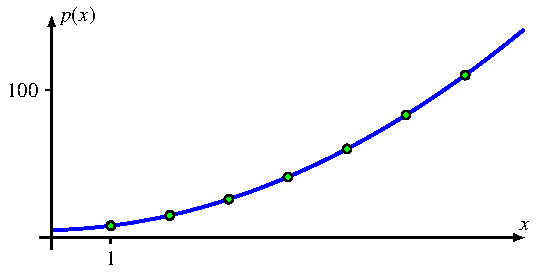
\includegraphics[scale = 1.2]{images/polynom1.pdf}}
		\only<2>{
			Versende $ (p(1),p(2),\dots,p(7)) = (\textcolor{green}{8}, 
			\textcolor{red}{50}, \textcolor{red}{37},
			\textcolor{green}{41}, \textcolor{green}{60}, 
			\textcolor{green}{83}, \textcolor{green}{110})$
			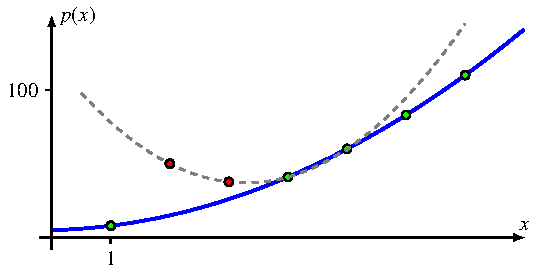
\includegraphics[scale = 1.2]{images/polynom2.pdf}
			\newline
			\textcolor{green}{7} Zahlen versenden, um \textcolor{blue}{3} Zahlen gegen \textcolor{red}{2} Fehlern abzusichern.}
	\end{frame}
%-------------------------------------------------------------------------------	
	\begin{frame}
	\frametitle{Parameter}
	\begin{center}
		\begin{tabular}{ c c c } 
			\hline
			``Nutzlas´´ & Fehler & Versenden \\
			\hline 
			3 & 2 & 7 Werte eines Polynoms vom Grad 2 \\ 
			4 & 2 & 8 Werte eines Polynoms vom Grad 3 \\
\visible<2->{3}& 
\visible<2->{3}& 
\visible<3->{9 Werte eines Polynoms vom Grad 2} \\ 
			&&\\
\visible<4->{$k$} & 
\visible<4->{$t$} & 
\visible<4->{$k+2t$ Werte eines Polynoms vom Grad $k-1$} \\ 
			\hline
			&&\\
			&&\\
			\multicolumn{3}{l} {
				\visible<4>{Ausserdem können bis zu $2t$ Fehler erkannt werden!}
			}
		\end{tabular}
	\end{center}	
	\end{frame}

%-------------------------------------------------------------------------------	

\section{Diskrete Fourier Transformation}
	\begin{frame}
		\frametitle{Idee}
		\begin{itemize}
			\item Fourier-transformieren
			\item Übertragung
			\item Rücktransformieren
		\end{itemize}
	\end{frame}
%-------------------------------------------------------------------------------	
	\begin{frame}
		\begin{figure}
			\only<1>{
			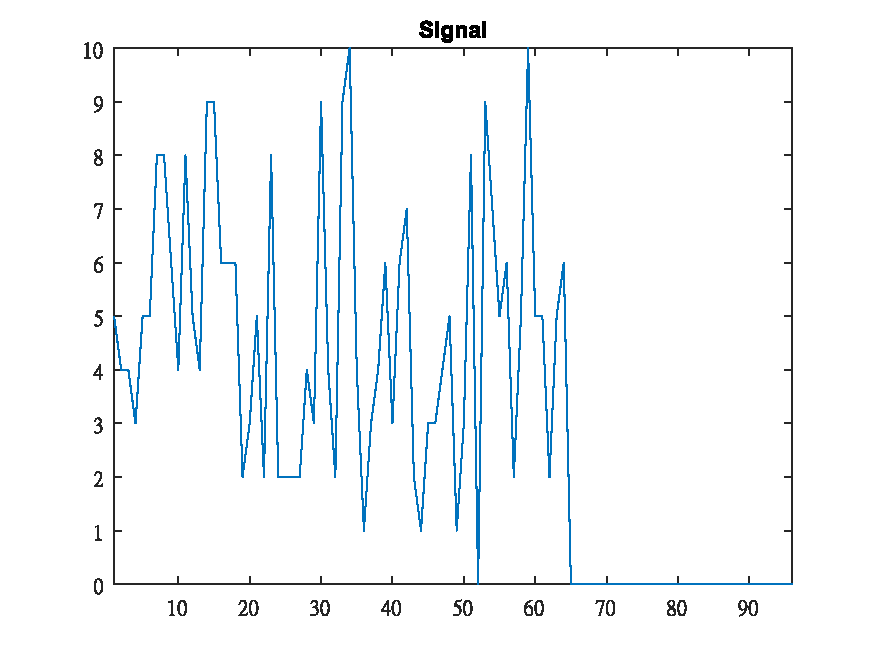
\includegraphics[width=0.9\linewidth]{images/fig1.pdf}
			}
			\only<2>{
			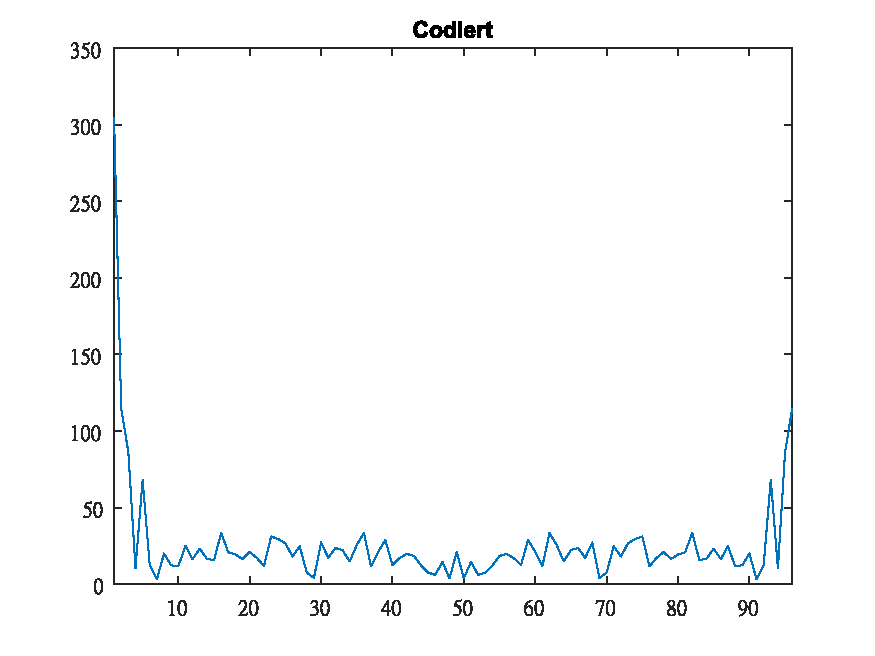
\includegraphics[width=0.9\linewidth]{images/fig2.pdf}
			}
			\only<3>{
			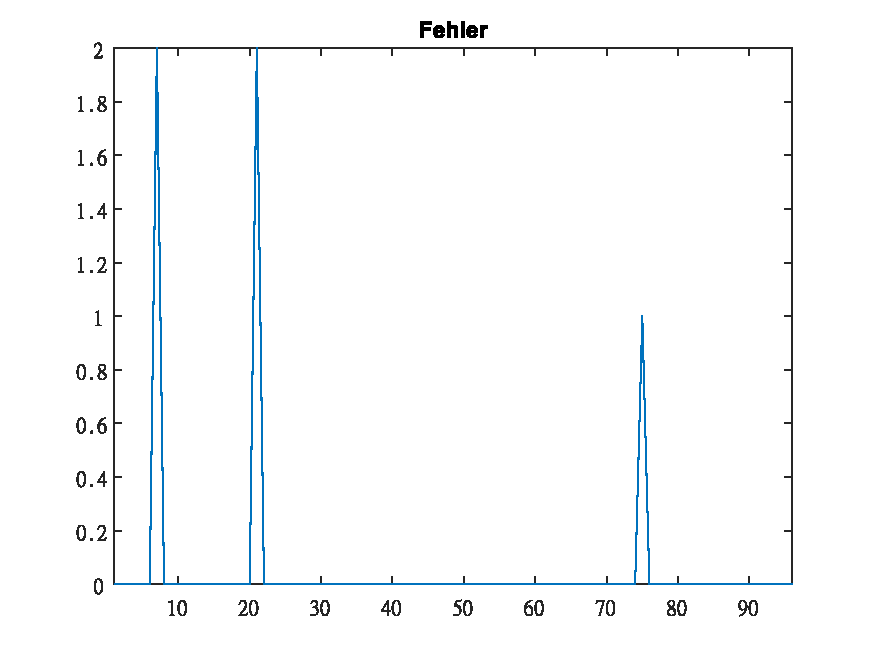
\includegraphics[width=0.9\linewidth]{images/fig3.pdf}
			}
			\only<4>{
			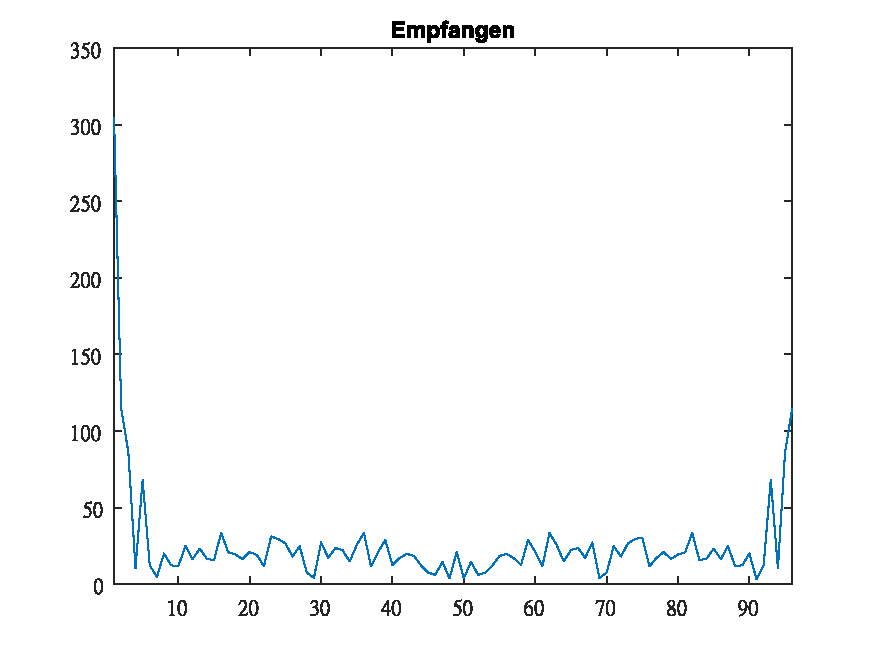
\includegraphics[width=0.9\linewidth]{images/fig4.pdf}
			}
			\only<5>{
			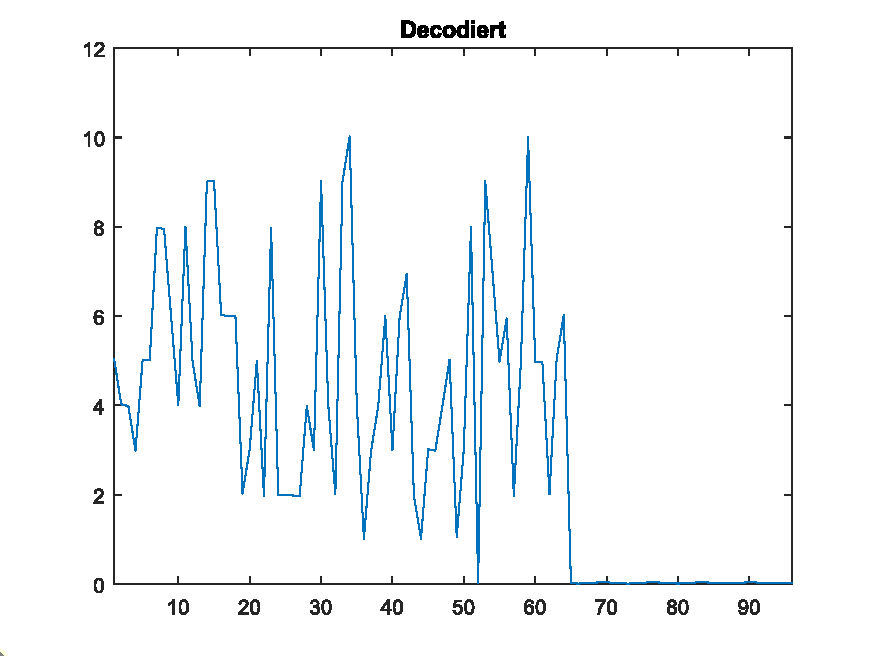
\includegraphics[width=0.9\linewidth]{images/fig5.pdf}
			}
			\only<6>{
			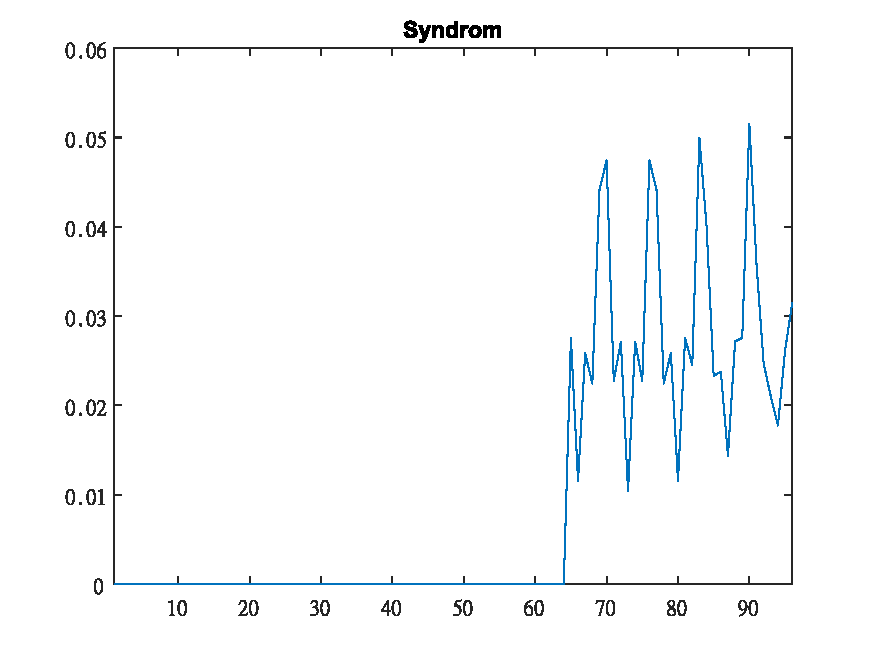
\includegraphics[width=0.9\linewidth]{images/fig6.pdf}
			}
			\only<7>{
			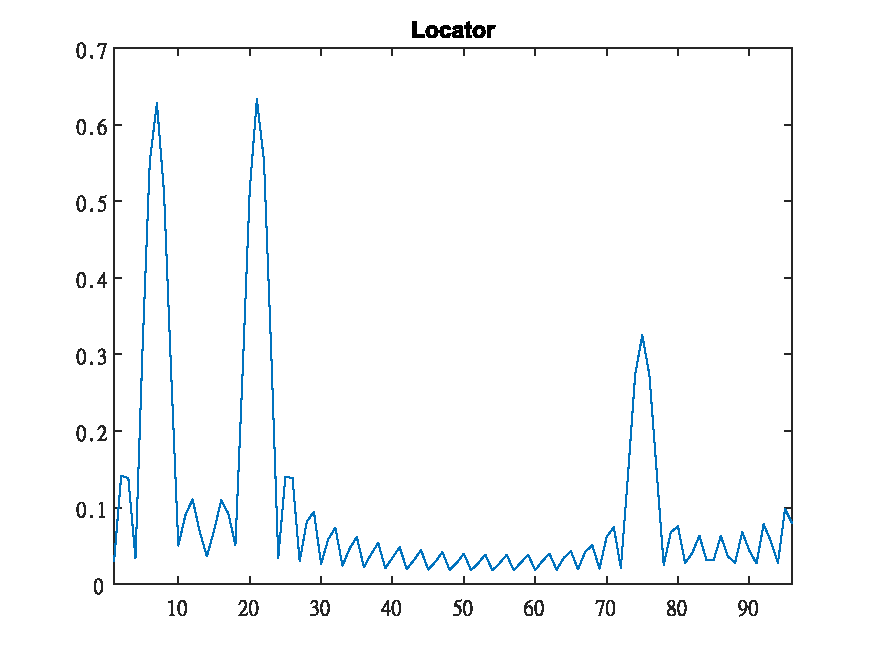
\includegraphics[width=0.9\linewidth]{images/fig7.pdf}
			}
	\end{figure}
	\end{frame}
%-------------------------------------------------------------------------------		
	\begin{frame}
	\frametitle{Diskrete Fourier Transformation}
	\begin{itemize}
	\item Diskrete Fourier-Transformation gegeben durch:
	\visible<1->{
	\[
	\label{ft_discrete}
	\hat{c}_{k} 
	= \frac{1}{N} \sum_{n=0}^{N-1}
	{f}_n \cdot e^{-\frac{2\pi j}{N} \cdot kn}
	\]}
	\visible<2->{
	\item Ersetzte
	\[
	w = e^{-\frac{2\pi j}{N} k}
	\]}
	\visible<3->{
	\item Wenn $N$ konstant:
	\[
	\hat{c}_{k}=\frac{1}{N}( {f}_0 w^0 + {f}_1 w^1 + {f}_2 w^2 + \dots + {f}_{N-1} w^N)
	\]}
	\end{itemize}
	\end{frame}	

%-------------------------------------------------------------------------------	
	\begin{frame}
	\frametitle{Diskrete Fourier Transformation}
	\[
	\begin{pmatrix}
		\hat{c}_1 \\\hat{c}_2 \\\hat{c}_3 \\ \vdots \\\hat{c}_n
	\end{pmatrix}
	= \frac{1}{N}
	\begin{pmatrix}
		w^0 & w^0   & w^0  & \dots  &w^0     \\
		w^0 & w^1   &w^2   & \dots  &w^{N-1}     \\ 
		w^0 & w^2   &w^4   & \dots  &w^{2(N-1)}  \\ 
		\vdots   & \vdots     &\vdots     &\ddots  &\vdots       \\
		w^0 & w^{1(N-1)}&w^{2(N-1)}& \dots  &w^{(N-1)(N-1)}  \\ 
	\end{pmatrix}
	\begin{pmatrix}
		\textcolor{blue}{f_0}  	\\
		\textcolor{blue}{f_1}	\\
		\textcolor{blue}{f_2}	\\	 
 		\vdots  \\
	 	0  \\ 
	\end{pmatrix}
	\]
	\end{frame}
%-------------------------------------------------------------------------------	

	\begin{frame}
		\frametitle{Probleme und Fragen}
		
			Wie wird der Fehler lokalisiert?
		\visible<2>{
			\newline
			Indem in einem endlichen Körper gerechnet wird.
		}
	\end{frame}	

%-------------------------------------------------------------------------------	


\section{Reed-Solomon in Endlichen Körpern}	

	\begin{frame}
		\frametitle{Reed-Solomon in Endlichen Körpern}
		
		\begin{itemize}
			\onslide<1->{\item Warum endliche Körper?}
			
			\onslide<1->{\qquad konkrete Zahlen $\rightarrow$ keine Rundungsfehler}
			
			\onslide<1->{\qquad digitale Fehlerkorrektur}
			
			\onslide<1->{\qquad bessere Laufzeit}
			
			\vspace{10pt}
			
			\onslide<1->{\item Nachricht = Nutzdaten + Fehlerkorrekturteil}
			
			\vspace{10pt}
			
			\onslide<1->{\item aus Fehlerkorrekturteil die Fehlerstellen finden}
			
			\onslide<1->{\qquad $\Rightarrow$ gesucht ist ein Lokatorpolynom}
			
%			\vspace{10pt}
			
%			\onslide<1->{\item Im Fehlerfall sollen wir aus der Nachricht ein Lokatorpolynom berechnen können, welches die fehlerhaften Stellen beinhaltet}
			
%			Wir sollten im Fehlerfall in der Lage sein, aus der Nachricht ein Lokatorpolynom zu berechnen, welches die Fehlerhaften Stellen beinhaltet
						
		\end{itemize}
		
%		TODO
		
%		erklärung und einführung der endlichen körper, was wollen wir erreichen?
		
%		wir versenden im endefekt mehr daten als unsere nachricht umfasst, damit die korrektur sichergestellt werden kann
		
%		sollten wir fehler bekommen, was uns die korrekturstellen mitgeteilt wird, dann ist es unsere aufgabe ein lokatorpolynom zu finden, welches uns verrät, auf welchen zeilen der Fehler aufgetreten ist
	\end{frame}
%-------------------------------------------------------------------------------
	\begin{frame}
		\frametitle{Definition eines Beispiels}
		
		\begin{itemize}
			
			\only<1->{\item endlicher Körper $q = 11$}
			
			\only<1->{ist eine Primzahl}

			\only<1->{beinhaltet die Zahlen $\mathbb{F}_{11} = \{0,1,2,3,4,5,6,7,8,9,10\}$}
			
			\vspace{10pt}
			
			\only<1->{\item Nachrichtenblock $=$ Nutzlast $+$ Fehlerkorrekturstellen
			
			$n = q - 1 = 10$ Zahlen}
			
			\vspace{10pt}
			
			\only<1->{\item Max.~Fehler $z = 2$
			
			maximale Anzahl von Fehler, die wir noch korrigieren können}
			
			\vspace{10pt}
			
			\only<1->{\item Nutzlast $k = n -2t = 6$ Zahlen}
			
			\only<1->{Fehlerkorrkturstellen $2t = 4$ Zahlen}
			
			\only<1->{Nachricht $m = [0,0,0,0,4,7,2,5,8,1]$}
			
			\only<1->{als Polynom $m(X) = 4X^5 + 7X^4 + 2X^3 + 5X^2 + 8X + 1$}
			
		\end{itemize}
		
	\end{frame}
%-------------------------------------------------------------------------------	
\section{Codierung eines Beispiels}
	\begin{frame}
		\frametitle{Codierung}
		
		\begin{itemize}
			\only<1->{\item Ansatz aus den komplexen Zahlen mit der diskreten Fouriertransformation}
			
			\vspace{10pt}
			
			\only<1->{\item Eulersche Zahl $\mathrm{e}$ existiert nicht in $\mathbb{F}_{11}$}
			
			\vspace{10pt}
			
			\only<1->{\item Wir suchen $a$ so, dass $a^i$ den gesamten Zahlenbereich von $\mathbb{F}_{11}$ abdecken
			
			$\mathbb{Z}_{11}\setminus\{0\} = \{a^0, a^1, a^2, a^3, a^4, a^5, a^6, a^7, a^8, a^9\}$}
			
			\vspace{10pt}
			
			\only<1->{\item Wir wählen $a = 8$}
			
			\only<1->{$\mathbb{Z}_{11}\setminus\{0\} = \{1,8,9,6,4,10,3,2,5,7\}$}
			
			\only<1->{$8$ ist eine primitive Einheitswurzel}
			
			\vspace{10pt}
			
			\only<1->{\item $m(8^0) = 4\cdot1 + 7\cdot1 + 2\cdot1 + 5\cdot1 + 8\cdot1 + 1 = 5$}
			
			\only<1->{$\Rightarrow$ \qquad können wir auch als Matrix schreiben}
			
		\end{itemize}
		
	\end{frame}
%-------------------------------------------------------------------------------		
	\begin{frame}
		\frametitle{Codierung}
		
		\begin{itemize}
			\only<1->{\item Übertragungsvektor $v$}
			
			\only<1->{\item $v = A \cdot m$}
			
		\end{itemize}
		
		\[
		\only<1->{
		v = \begin{pmatrix}
			8^0&    8^0&    8^0&    8^0&    8^0&    8^0&    8^0&    8^0&    8^0&    8^0\\
			8^0&	8^1&	8^2&	8^3&	8^4&	8^5&	8^6&	8^7&    8^8&	8^9\\
			8^0&	8^2&	8^4&	8^6&	8^8& 8^{10}& 8^{12}& 8^{14}& 8^{16}& 8^{18}\\
			8^0&	8^3&	8^6&	8^9& 8^{12}& 8^{15}& 8^{18}& 8^{21}& 8^{24}& 8^{27}\\
			8^0&	8^4&	8^8& 8^{12}& 8^{16}& 8^{20}& 8^{24}& 8^{28}& 8^{32}& 8^{36}\\
			8^0&	8^5& 8^{10}& 8^{15}& 8^{20}& 8^{25}& 8^{30}& 8^{35}& 8^{40}& 8^{45}\\
			8^0&	8^6& 8^{12}& 8^{18}& 8^{24}& 8^{30}& 8^{36}& 8^{42}& 8^{48}& 8^{54}\\
			8^0&	8^7& 8^{14}& 8^{21}& 8^{28}& 8^{35}& 8^{42}& 8^{49}& 8^{56}& 8^{63}\\
			8^0&	8^8& 8^{16}& 8^{24}& 8^{32}& 8^{40}& 8^{48}& 8^{56}& 8^{64}& 8^{72}\\
			8^0&	8^9& 8^{18}& 8^{27}& 8^{36}& 8^{45}& 8^{54}& 8^{63}& 8^{72}& 8^{81}\\
		\end{pmatrix}
		\cdot
		\begin{pmatrix}
			1 \\ 8 \\ 5 \\ 2 \\ 7 \\ 4 \\ 0 \\ 0 \\ 0 \\ 0 \\
		\end{pmatrix}
		}
		\]
		\only<1->{
		\begin{itemize}
			\item $v = [5,3,6,5,2,10,2,7,10,4]$
		\end{itemize}
		}	
	\end{frame}
%-------------------------------------------------------------------------------	
\section{Decodierung ohne Fehler}
	\begin{frame}
		\frametitle{Decodierung ohne Fehler}
		
		\begin{itemize}
			\only<1->{\item Der Empfänger erhält den unveränderten Vektor 
			$v = [5,3,6,5,2,10,2,7,10,4]$}
			
			\vspace{10pt}
			
			\only<1->{\item Wir suchen die Inverse der Matrix $A$}
			
			\vspace{10pt}
			
		\end{itemize}
		
		\begin{columns}[t]
		\begin{column}{0.50\textwidth}		
		\only<1->{
		Inverse der Fouriertransformation
		\vspace{10pt}
		\[
		F(\omega) = \int_{-\infty}^{\infty} f(t) \mathrm{e}^{-j\omega t} dt
		\]
		\vspace{10pt}
		\[
		\mathfrak{F}^{-1}(F(\omega)) = f(t) = \frac{1}{2 \pi} \int_{-\infty}^{\infty} F(\omega) \mathrm{e}^{j \omega t} d\omega
		\]
		}
		\end{column}
		\begin{column}{0.50\textwidth}		
		\only<1->{
		Inverse von $a$}
		\vspace{10pt}
		\only<1->{
		\[
		8^{1} \Rightarrow 8^{-1}
		\]
		}
		\only<1->{Inverse finden wir über den Eulkidischen Algorithmus}
		\vspace{10pt}
		\end{column}
		\end{columns}		
		
	\end{frame}
%-------------------------------------------------------------------------------		
	\begin{frame}
		\frametitle{Der Euklidische Algorithmus}
	
	\begin{columns}[t]
	\begin{column}{0.50\textwidth}	
	
	Recap aus der Vorlesung:
	
	Gegeben $a \in \mathbb{F}_p$, finde $b = a^{-1} \in \mathbb{F}_p$
	
	\begin{tabular}{rcl}
		$a  b$ &$\equiv$& $1 \mod p$\\
		$a  b$ &$=$& $1 + n  p$\\
		$a  b - n  p$ &$=$& $1$\\
		&&\\
		$\operatorname{ggT}(a,p)$&$=$& $1$\\
		$sa + tp$&$=$& $1$\\
		$b$&$=$&$s$\\
		$n$&$=$&$-t$
	\end{tabular}
	
	\end{column}
	\begin{column}{0.50\textwidth}	
	
	\begin{center}
	\only<1->{
	\begin{tabular}{| c | c c | c | r r |}
		\hline
		$k$ & $a_i$ & $b_i$ & $q_i$ & $c_i$ & $d_i$\\
		\hline 
		& & & & $1$& $0$\\
		$0$& $8$& $11$& $0$& $0$& $1$\\
		$1$& $11$& $8$& $1$& $1$& $0$\\
		$2$& $8$& $3$& $2$& $-1$& $1$\\
		$3$& $3$& $2$& $1$& $3$& $-2$\\
		$4$& $2$& $1$& $2$& \textcolor<3->{blue}{$-4$}& \textcolor<3->{red}{$3$}\\
		$5$& $1$& $0$& & $11$& $-8$\\
		\hline
	\end{tabular}	
	}
	\vspace{10pt}
	
	\begin{tabular}{rcl}
		\only<1->{$\textcolor{blue}{-4} \cdot 8 + \textcolor{red}{3} \cdot 11$ &$=$& $1$}\\
		\only<1->{$7 \cdot 8 + 3 \cdot 11$ &$=$& $1$}\\
		\only<1->{$8^{-1}$ &$=$& $7$}
		
	\end{tabular}
	
	\end{center}
	
	\end{column}
	\end{columns}
	
	\end{frame}
%-------------------------------------------------------------------------------	
	\begin{frame}
		\frametitle{Decodierung mit Inverser Matrix}	
		
		\begin{itemize}
			\only<1->{\item $v = [5,3,6,5,2,10,2,7,10,4]$}
			
			\only<1->{\item $m = 1/10 \cdot A^{-1} \cdot v$}
			
			\only<1->{\item $m = 10 \cdot A^{-1} \cdot v$}
			
		\end{itemize}
		\only<1->{
		\[
		m = \begin{pmatrix}
			7^0&    7^0&    7^0&    7^0&    7^0&    7^0&    7^0&    7^0&    7^0&    7^0\\
			7^0&	7^1&	7^2&	7^3&	7^4&	7^5&	7^6&	7^7&    7^8&	7^9\\
			7^0&	7^2&	7^4&	7^6&	7^8& 7^{10}& 7^{12}& 7^{14}& 7^{16}& 7^{18}\\
			7^0&	7^3&	7^6&	7^9& 7^{12}& 7^{15}& 7^{18}& 7^{21}& 7^{24}& 7^{27}\\
			7^0&	7^4&	7^8& 7^{12}& 7^{16}& 7^{20}& 7^{24}& 7^{28}& 7^{32}& 7^{36}\\
			7^0&	7^5& 7^{10}& 7^{15}& 7^{20}& 7^{25}& 7^{30}& 7^{35}& 7^{40}& 7^{45}\\
			7^0&	7^6& 7^{12}& 7^{18}& 7^{24}& 7^{30}& 7^{36}& 7^{42}& 7^{48}& 7^{54}\\
			7^0&	7^7& 7^{14}& 7^{21}& 7^{28}& 7^{35}& 7^{42}& 7^{49}& 7^{56}& 7^{63}\\
			7^0&	7^8& 7^{16}& 7^{24}& 7^{32}& 7^{40}& 7^{48}& 7^{56}& 7^{64}& 7^{72}\\
			7^0&	7^9& 7^{18}& 7^{27}& 7^{36}& 7^{45}& 7^{54}& 7^{63}& 7^{72}& 7^{81}\\
		\end{pmatrix}
		\cdot
		\begin{pmatrix}
			5 \\ 3 \\ 6 \\ 5 \\ 2 \\ 10 \\ 2 \\ 7 \\ 10 \\ 4 \\
		\end{pmatrix}
		\]
		}
		\only<1->{
		\begin{itemize}
			\item $m = [0,0,0,0,4,7,2,5,8,1]$
		\end{itemize}
		}
	\end{frame}
%-------------------------------------------------------------------------------		
\section{Decodierung mit Fehler}
	\begin{frame}
		\frametitle{Decodierung mit Fehler - Ansatz}	
		
		\begin{itemize}
			\only<1->{\item Gesendet: $v = [5,3,6,5,2,10,2,7,10,4]$}
			
			\only<1->{\item Empfangen: $w = [5,3,6,\textcolor{red}{8},2,10,2,7,\textcolor{red}{1},4]$}
			
			\only<1->{\item Rücktransformation: $r = [\underbrace{5,7,4,10,}_{Fehlerinfo}5,4,5,7,6,7]$}
			
		\end{itemize}
		
	\only<1->{Wie finden wir die Fehler?}
		
		\only<1->{
		\begin{itemize}
			\item $m(X) = 4X^5 + 7X^4 + 2X^3 + 5X^2 + 8X + 1$
			
			\item $r(X) = 5X^9 + 7X^8 + 4X^7 + 10X^6 + 5X^5 + 4X^4 + 5X^3 + 7X^2 + 6X + 7$
			
			%\only<7->{\item $e(X) = r(X) - m(X)$}
			
			\item $e(X) = r(X) - m(X)$
			
		\end{itemize}	
	}

		\begin{center}
			\only<1->{
		\begin{tabular}{c c c c c c c c c c c}
			\hline
			$i$& $0$& $1$& $2$& $3$& $4$& $5$& $6$& $7$& $8$& $9$\\
			\hline
			$r(a^{i})$& \only<1->{$5$& $3$& $6$& $8$& $2$& $10$& $2$& $7$& $1$& $4$}\\
			$m(a^{i})$& \only<1->{$5$& $3$& $6$& $5$& $2$& $10$& $2$& $7$& $10$& $4$}\\
			$e(a^{i})$& \only<1->{$0$& $0$& $0$& $3$& $0$& $0$& $0$& $0$& $2$& $0$}\\
			\hline
		\end{tabular}	
			}
		\end{center}
	
		\only<1->{
		\begin{itemize}
			\item Alle Stellen, die nicht Null sind, sind Fehler
		\end{itemize}
		}

	\end{frame}
%-------------------------------------------------------------------------------		
	\begin{frame}
		\frametitle{Nullstellen des Fehlerpolynoms finden}
		
		\begin{itemize}
			\only<1->{\item Satz von Fermat: $f(X) = X^{q-1}-1=0$}
			
			\vspace{10pt}
			
			\only<1->{\item $f(X) = X^{10}-1 = 0$ \qquad für $X \in \{1,2,3,4,5,6,7,8,9,10\}$}
			
			\vspace{10pt}
			
			\only<1->{\item $f(X) = (X-a^0)(X-a^1)(X-a^2)(X-a^3)(X-a^4)(X-a^5)(X-a^6) \cdot$
			
			\qquad \qquad $(X-a^7)(X-a^8)(X-a^9)$}
			
			\vspace{10pt}
			
			\only<1->{\item $e(X) = (X-a^0)(X-a^1)(X-a^2) \qquad \qquad (X-a^4)(X-a^5)(X-a^6) \cdot$
			
			\qquad \qquad $(X-a^7) \qquad \qquad (X-a^9) \cdot p(x)$}
			
			\vspace{10pt}
			
			\only<1->{\item $\operatorname{ggT}$ gibt uns eine Liste der Nullstellen, an denen es keine Fehler gegeben hat}
			
			\vspace{10pt}
			
			\only<1->{$\operatorname{ggT}(f(X),e(X)) = (X-a^0)(X-a^1)(X-a^2) \qquad \qquad (X-a^4)(X-a^5)(X-a^6) \cdot$
			
			\qquad \qquad \qquad \qquad $(X-a^7) \qquad \qquad (X-a^9)$}
				
		\end{itemize}
			
	\end{frame}
%-------------------------------------------------------------------------------	
	\begin{frame}
		\frametitle{Nullstellen des Fehlerpolynoms finden}
		
		\begin{itemize}
			
			\item Satz von Fermat: $f(X) = X^{q-1}-1=0$
			
			\vspace{10pt}
			
			\item $f(X) = X^{10}-1 = 0$ \qquad für $X = [1,2,3,4,5,6,7,8,9,10]$
			
			\vspace{10pt}
			
			\item $f(X) = (X-a^0)(X-a^1)(X-a^2)(X-a^3)(X-a^4)(X-a^5)(X-a^6) \cdot$
			
			\qquad \qquad $(X-a^7)(X-a^8)(X-a^9)$
			
			\vspace{10pt}
			
			\item $e(X) = (X-a^0)(X-a^1)(X-a^2) \qquad \qquad (X-a^4)(X-a^5)(X-a^6) \cdot$
			
			\qquad \qquad $(X-a^7) \qquad \qquad (X-a^9) \cdot p(x)$
			
			\vspace{10pt}
			
			\item $\operatorname{kgV}$ gibt uns eine Liste von aller Nullstellen, die wir in $e$ und $d$ zerlegen können
			
			\vspace{10pt}
			
			$\operatorname{kgV}(f(X),e(X)) = (X-a^0)(X-a^1)(X-a^2)(X-a^3)(X-a^4)(X-a^5)(X-a^6) \cdot $
			
			\qquad \qquad \qquad \qquad $(X-a^7)(X-a^8)(X-a^9) \cdot q(X)$
			
			$= d(X) \cdot e(X)$
			
			\vspace{10pt}
			
			\item Lokatorpolynom $d(X) = (X-a^3)(X-a^8)$
			
		\end{itemize}
	
	\end{frame}
%-------------------------------------------------------------------------------	
	\begin{frame}
		\frametitle{Kennen wir $e(X)$?}
		
		\begin{itemize}
			
			\only<1->{\item $e(X)$ ist unbekannt auf der Empfängerseite}
			
			\vspace{10pt}
			
			\only<1->{\item $e(X) = r(X) - m(X)$ \qquad $\rightarrow$ \qquad $m(X)$ ist unbekannt?}
			
			\vspace{10pt}
			
			\only<1->{\item $m$ ist nicht gänzlich unbekannt: $m = [0,0,0,0,?,?,?,?,?,?]$
			
			In den bekannten Stellen liegt auch die Information, wo es Fehler gegeben hat}
			
			\vspace{10pt}
			
			\only<1->{\item Daraus folgt $e(X) = 5X^9 + 7X^8 + 4X^7 + 10X^6 + p(X)$}
			
			\vspace{10pt}
			
			\only<1->{\item $f(X) = X^{10} - 1 = X^{10} + 10$}
			
			\vspace{10pt}
			
			\only<1->{\item Jetzt können wir den $\operatorname{ggT}$ von $f(X)$ und $e(X)$ berechnen}
		\end{itemize}
		
	\end{frame}
%-------------------------------------------------------------------------------	
	\begin{frame}
		\frametitle{Der Euklidische Algorithmus (nochmal)}
		
		\only<1->{$\operatorname{ggT}(f(X),e(X))$ hat den Grad $8$}
		\only<1->{
		\[
		\arraycolsep=1.4pt
		\begin{array}{rcrcrcrcccrcrcrcrcrcrcrcrcr}
			X^{10}& & & & & & &+& 10& & & & &:&5X^9&+&7X^8&+& 4X^7&+&10X^6&+&p(X)&=&9X&+&5\\
			X^{10}&+& 8X^9&+& 3X^8&+&2X^7&+& p(X)& &  & & & &   & & & & & &   & &  & & \\ \cline{1-9}
			&& 3X^9&+& 8X^8&+& 9X^7&+& p(X)& &   & & & & & &   & &  & & \\
			&& 3X^9&+& 2X^8&+& 9X^7&+& p(X)& &   & & & & & &   & &  & & \\ \cline{3-9}
			& &    & &6X^8&+&0X^7&+&p(X)& &   & & & & & &   & &  & & \\
		\end{array}
		\]
		}
		\only<1->{
		\[
		\arraycolsep=1.4pt
		\begin{array}{rcrcrcrcccrcrcrcrcrcrcrcrcr}
			5X^9&+& 7X^8&+& 4X^7&+& 10X^6&+& p(X)& & & & &:&6X^8&+&0X^7& & & & & & &=&10X&+&3\\
			5X^9&+& 0X^8&+& p(X)& & & & & &  & & & &   & & & & & &   & &  & & \\ \cline{1-5}
			&& 7X^8&+& p(X)& & & & & &   & & & & & &   & &  & & \\
		\end{array}
		\]
		}
		\vspace{10pt}
		
		\only<1->{$\operatorname{ggT}(f(X),e(X)) = 6X^8$}
		
		\vspace{10pt}
		
		\only<1->{	$\operatorname{kgV}$ durch den erweiterten Euklidischen Algorithmus bestimmen	}
		
	\end{frame}
		
%-------------------------------------------------------------------------------	
	\begin{frame}
		\frametitle{Der Erweiterte Euklidische Algorithmus}
		
		\begin{center}
			
		\begin{tabular}{| c | c | c c |}
			\hline
			$k$ &  $q_i$ & $e_i$ & $f_i$\\
			\hline 
			& & $0$& $1$\\
			$0$& $9X + 5$& $1$& $0$\\
			$1$& $10X + 3$& $9X+5$& $1$\\
			$2$& & \textcolor<2->{blue}{$2X^2 + 0X + 5$}& $10X + 3$\\
			\hline
		\end{tabular}	
			
		\end{center}
		
		\vspace{10pt}
		
		\begin{tabular}{ll}
			\only<1->{Somit erhalten wir den Faktor& $d(X) = 2X^2 + 5$\\}
			\only<1->{Faktorisiert erhalten wir& $d(X) = 2(X-5)(X-6)$\\}
			\only<1->{Lokatorpolynom& $d(X) = (X-a^i)(X-a^i)$}
		\end{tabular}
		
		\vspace{10pt}
		\only<1->{
		\begin{center}
			$a^i = 5 \qquad \Rightarrow \qquad i = 3$
			
			$a^i = 6 \qquad \Rightarrow \qquad i = 8$
		\end{center}
	}
	\only<1->{$d(X) = (X-a^3)(X-a^8)$}
		
	\end{frame}
%-------------------------------------------------------------------------------	
\section{Nachricht Rekonstruieren}	
	\begin{frame}
		\frametitle{Rekonstruktion der Nachricht}
		
		\begin{itemize}
			
			\only<1->{\item $w = [5,3,6,8,2,10,2,7,1,4]$}
			
			\only<1->{\item $d(X) = (X-\textcolor<4->{red}{a^3})(X-\textcolor<4->{red}{a^8})$}
			
		\end{itemize}
		\only<1->{
		\[
		\textcolor{gray}{
		\begin{pmatrix}
			 a^0 \\ a^1 \\ a^2 \\ \textcolor<4->{red}{a^3} \\ a^4 \\ a^5 \\ a^6 \\ a^7 \\ \textcolor<4->{red}{a^8} \\ a^9 \\
		\end{pmatrix}}
		\begin{pmatrix}
			5 \\ 3 \\ 6 \\ \textcolor<4->{red}{8} \\ 2 \\ 10 \\ 2 \\ 7 \\ \textcolor<4->{red}{1} \\ 4 \\
		\end{pmatrix}
		=
		\begin{pmatrix}
			8^0&    8^0&    8^0&    8^0&    8^0&    8^0&    8^0&    8^0&    8^0&    8^0\\
			8^0&	8^1&	8^2&	8^3&	8^4&	8^5&	8^6&	8^7&    8^8&	8^9\\
			8^0&	8^2&	8^4&	8^6&	8^8& 8^{10}& 8^{12}& 8^{14}& 8^{16}& 8^{18}\\
			\textcolor<4->{red}{8^0}&	\textcolor<4->{red}{8^3}&	\textcolor<4->{red}{8^6}&	\textcolor<4->{red}{8^9}& \textcolor<4->{red}{8^{12}}& \textcolor<4->{red}{8^{15}}& \textcolor<4->{red}{8^{18}}& \textcolor<4->{red}{8^{21}}& \textcolor<4->{red}{8^{24}}& \textcolor<4->{red}{8^{27}}\\
			8^0&	8^4&	8^8& 8^{12}& 8^{16}& 8^{20}& 8^{24}& 8^{28}& 8^{32}& 8^{36}\\
			8^0&	8^5& 8^{10}& 8^{15}& 8^{20}& 8^{25}& 8^{30}& 8^{35}& 8^{40}& 8^{45}\\
			8^0&	8^6& 8^{12}& 8^{18}& 8^{24}& 8^{30}& 8^{36}& 8^{42}& 8^{48}& 8^{54}\\
			8^0&	8^7& 8^{14}& 8^{21}& 8^{28}& 8^{35}& 8^{42}& 8^{49}& 8^{56}& 8^{63}\\
			\textcolor<4->{red}{8^0}&	\textcolor<4->{red}{8^8}& \textcolor<4->{red}{8^{16}}& \textcolor<4->{red}{8^{24}}& \textcolor<4->{red}{8^{32}}& \textcolor<4->{red}{8^{40}}& \textcolor<4->{red}{8^{48}}& \textcolor<4->{red}{8^{56}}& \textcolor<4->{red}{8^{64}}& \textcolor<4->{red}{8^{72}}\\
			8^0&	8^9& 8^{18}& 8^{27}& 8^{36}& 8^{45}& 8^{54}& 8^{63}& 8^{72}& 8^{81}\\
		\end{pmatrix}
		\cdot
		\begin{pmatrix}
			m_0 \\ m_1 \\ m_2 \\ m_3 \\ m_4 \\ m_5 \\ m_6 \\ m_7 \\ m_8 \\ m_9 \\
		\end{pmatrix}
		\]
		}
		\only<1->{
		\begin{itemize}
			\item Fehlerstellen entfernen
		\end{itemize}
		}
	\end{frame}	
%-------------------------------------------------------------------------------		
	\begin{frame}
		\frametitle{Rekonstruktion der Nachricht}
		
		\[
		\begin{pmatrix}
			5 \\ 3 \\ 6 \\ 2 \\ 10 \\ 2 \\ 7 \\ 4 \\
		\end{pmatrix}
		=
		\begin{pmatrix}
			8^0&    8^0&    8^0&    8^0&    8^0&    8^0&    \textcolor<3->{green}{8^0}&    \textcolor<3->{green}{8^0}&    \textcolor<3->{green}{8^0}&    \textcolor<3->{green}{8^0}\\
			8^0&	8^1&	8^2&	8^3&	8^4&	8^5&	\textcolor<3->{green}{8^6}&	 \textcolor<3->{green}{8^7}&     \textcolor<3->{green}{8^8}&	  \textcolor<3->{green}{8^9}\\
			8^0&	8^2&	8^4&	8^6&	8^8& 8^{10}& \textcolor<3->{green}{8^{12}}& \textcolor<3->{green}{8^{14}}& \textcolor<3->{green}{8^{16}}& \textcolor<3->{green}{8^{18}}\\
			8^0&	8^4&	8^8& 8^{12}& 8^{16}& 8^{20}& \textcolor<3->{green}{8^{24}}& \textcolor<3->{green}{8^{28}}& \textcolor<3->{green}{8^{32}}& \textcolor<3->{green}{8^{36}}\\
			8^0&	8^5& 8^{10}& 8^{15}& 8^{20}& 8^{25}& \textcolor<3->{green}{8^{30}}& \textcolor<3->{green}{8^{35}}& \textcolor<3->{green}{8^{40}}& \textcolor<3->{green}{8^{45}}\\
			8^0&	8^6& 8^{12}& 8^{18}& 8^{24}& 8^{30}& \textcolor<3->{green}{8^{36}}& \textcolor<3->{green}{8^{42}}& \textcolor<3->{green}{8^{48}}& \textcolor<3->{green}{8^{54}}\\
			8^0&	8^7& 8^{14}& 8^{21}& 8^{28}& 8^{35}& \textcolor<3->{green}{8^{42}}& \textcolor<3->{green}{8^{49}}& \textcolor<3->{green}{8^{56}}& \textcolor<3->{green}{8^{63}}\\
			8^0&	8^9& 8^{18}& 8^{27}& 8^{36}& 8^{45}& \textcolor<3->{green}{8^{54}}& \textcolor<3->{green}{8^{63}}& \textcolor<3->{green}{8^{72}}& \textcolor<3->{green}{8^{81}}\\
		\end{pmatrix}
		\cdot
		\begin{pmatrix}
			m_0 \\ m_1 \\ m_2 \\ m_3 \\ m_4 \\ m_5 \\ \textcolor<2->{green}{m_6} \\ \textcolor<2->{green}{m_7} \\ \textcolor<2->{green}{m_8} \\ \textcolor<2->{green}{m_9} \\
		\end{pmatrix}
		\]
		\only<1->{
		\begin{itemize}
			\item Nullstellen entfernen
		\end{itemize}
	}
	\end{frame}
%-------------------------------------------------------------------------------
	\begin{frame}
		\frametitle{Rekonstruktion der Nachricht}
		
		\[
		\begin{pmatrix}
			5 \\ 3 \\ 6 \\ 2 \\ 10 \\ 2 \\ \textcolor<2->{red}{7} \\ \textcolor<2->{red}{4} \\
		\end{pmatrix}
		=
		\begin{pmatrix}
			8^0&    8^0&    8^0&    8^0&    8^0&    8^0\\
			8^0&	8^1&	8^2&	8^3&	8^4&	8^5\\
			8^0&	8^2&	8^4&	8^6&	8^8& 8^{10}\\
			8^0&	8^4&	8^8& 8^{12}& 8^{16}& 8^{20}\\
			8^0&	8^5& 8^{10}& 8^{15}& 8^{20}& 8^{25}\\
			8^0&	8^6& 8^{12}& 8^{18}& 8^{24}& 8^{30}\\
			\textcolor<2->{red}{8^0}&	\textcolor<2->{red}{8^7}& \textcolor<2->{red}{8^{14}}& \textcolor<2->{red}{8^{21}}& \textcolor<2->{red}{8^{28}}& \textcolor<2->{red}{8^{35}}\\
			\textcolor<2->{red}{8^0}&	\textcolor<2->{red}{8^9}& \textcolor<2->{red}{8^{18}}& \textcolor<2->{red}{8^{27}}& \textcolor<2->{red}{8^{36}}& \textcolor<2->{red}{8^{45}}\\
		\end{pmatrix}
		\cdot
		\begin{pmatrix}
			m_0 \\ m_1 \\ m_2 \\ m_3 \\ m_4 \\ m_5 \\
		\end{pmatrix}
		\]
		
		\vspace{5pt}
		\only<1->{
		\begin{itemize}
			\item Matrix in eine Quadratische Form bringen
		\end{itemize}
	}
	\end{frame}
%-------------------------------------------------------------------------------	
	\begin{frame}
		\frametitle{Rekonstruktion der Nachricht}
		
		\[
		\begin{pmatrix}
			5 \\ 3 \\ 6 \\ 2 \\ 10 \\ 2 \\
		\end{pmatrix}
		=
		\begin{pmatrix}
			8^0&    8^0&    8^0&    8^0&    8^0&    8^0\\
			8^0&	8^1&	8^2&	8^3&	8^4&	8^5\\
			8^0&	8^2&	8^4&	8^6&	8^8& 8^{10}\\
			8^0&	8^4&	8^8& 8^{12}& 8^{16}& 8^{20}\\
			8^0&	8^5& 8^{10}& 8^{15}& 8^{20}& 8^{25}\\
			8^0&	8^6& 8^{12}& 8^{18}& 8^{24}& 8^{30}\\
		\end{pmatrix}
		\cdot
		\begin{pmatrix}
			m_0 \\ m_1 \\ m_2 \\ m_3 \\ m_4 \\ m_5 \\
		\end{pmatrix}
		\]
		
		\vspace{5pt}
		
		\begin{itemize}
			\item Matrix Invertieren
		\end{itemize}
		
	\end{frame}
%-------------------------------------------------------------------------------
	\begin{frame}
		\frametitle{Rekonstruktion der Nachricht}
		
		\[
		\begin{pmatrix}
			5 \\ 3 \\ 6 \\ 2 \\ 10 \\ 2 \\
		\end{pmatrix}
		=
		\begin{pmatrix}
			1&  1& 1&  1& 1&  1\\
			1&  8& 9&  6& 4& 10\\
			1&  9& 4&  3& 5&  1\\
			1&  4& 5&  9& 3&  1\\
			1& 10& 1& 10& 1& 10\\
			1&  3& 9&  5& 4&  1\\
		\end{pmatrix}
		\cdot
		\begin{pmatrix}
			m_0 \\ m_1 \\ m_2 \\ m_3 \\ m_4 \\ m_5 \\
		\end{pmatrix}
		\]
		
		\begin{center}
			$\Downarrow$
		\end{center}
		\[
		\begin{pmatrix}
			m_0 \\ m_1 \\ m_2 \\ m_3 \\ m_4 \\ m_5 \\
		\end{pmatrix}
		=
		\begin{pmatrix}
			 6&  4&  4&  6& 2&  1\\
			 2&  7& 10&  3& 4&  7\\
			 1&  8&  9&  8& 3&  4\\
			 3&  6&  6&  4& 5&  9\\
			10& 10&  9&  8& 1&  6\\
			 1&  9&  6&  4& 7&  6\\
		\end{pmatrix}
		\cdot
		\begin{pmatrix}
			5 \\ 3 \\ 6 \\ 2 \\ 10 \\ 2 \\
		\end{pmatrix}
		\]
		
	\end{frame}
%-------------------------------------------------------------------------------
	\begin{frame}
		\frametitle{Rekonstruktion der Nachricht}
		
		\[
		\begin{pmatrix}
			m_0 \\ m_1 \\ m_2 \\ m_3 \\ m_4 \\ m_5 \\
		\end{pmatrix}
		=
		\begin{pmatrix}
			6&  4&  4&  6& 2&  1\\
			2&  7& 10&  3& 4&  7\\
			1&  8&  9&  8& 3&  4\\
			3&  6&  6&  4& 5&  9\\
			10& 10&  9&  8& 1&  6\\
			1&  9&  6&  4& 7&  6\\
		\end{pmatrix}
		\cdot
		\begin{pmatrix}
			5 \\ 3 \\ 6 \\ 2 \\ 10 \\ 2 \\
		\end{pmatrix}
		\]
		
		\begin{itemize}
			\item $m = [4,7,2,5,8,1]$
		\end{itemize}
		
	\end{frame}
%-------------------------------------------------------------------------------

\end{document}
